In questa appendice, si presenta come il valore di \textit{fitness} della soluzione globale ottima è cambiato durante il processo di ottimizzazione (Figura \ref{apxfig:optimalfitness}) e quali sono i valori che hanno permesso di ottenerlo (Tabella \ref{apxtab:vs}). 
\begin{figure}
	\centering
	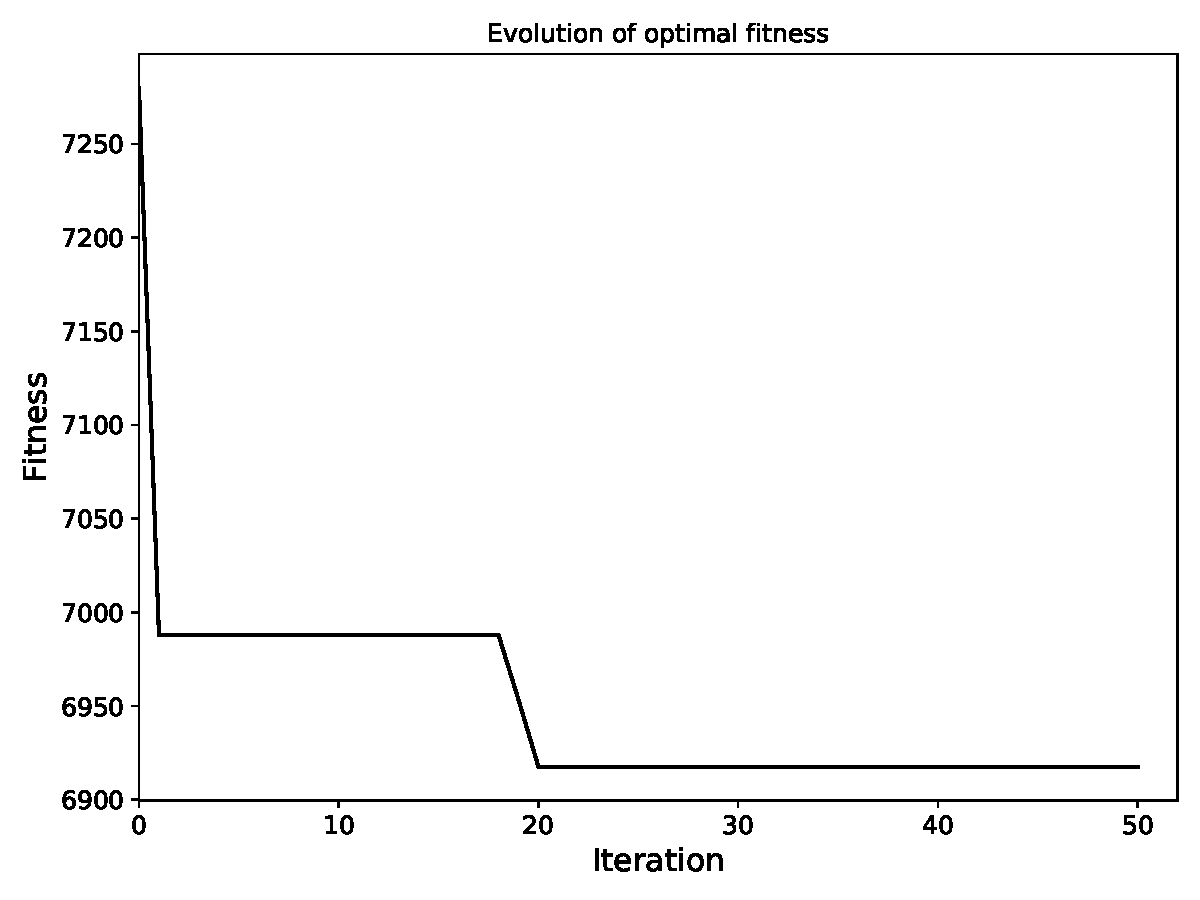
\includegraphics[width=0.9\linewidth]{images/optimal_fitness}
	\caption{Evoluzione del valore di \textit{fitness} della soluzione globale ottima individuavata, fino a quell'iterazione, dal processo di ottimizzazione.}
	\label{apxfig:optimalfitness}
\end{figure}
\begin{longtable}{c|c|c|c}
	\caption{Tabella rappresentante i valori assunti dai vari parametri che hanno portato a ottenere la soluzione globale ottima individuata, fino a quell'iterazione, dal processo di ottimizzazione.} \label{apxtab:vs} \\
	\textbf{numero di robot} & \textbf{raggio di percezione} & \textbf{$\alpha$} & \textbf{$\gamma$} \\
	\hline
	\endfirsthead 
	5.889 & 4.975 & 9.675 & 0.502 \\
	5.732 & 6.068 & 8.175 & 0.652 \\
	5.732 & 6.068 & 8.175 & 0.652 \\
	5.732 & 6.068 & 8.175 & 0.652 \\
	5.732 & 6.068 & 8.175 & 0.652 \\
	5.732 & 6.068 & 8.175 & 0.652 \\
	5.732 & 6.068 & 8.175 & 0.652 \\
	5.732 & 6.068 & 8.175 & 0.652 \\
	5.732 & 6.068 & 8.175 & 0.652 \\
	5.732 & 6.068 & 8.175 & 0.652 \\
	5.732 & 6.068 & 8.175 & 0.652 \\
	5.732 & 6.068 & 8.175 & 0.652 \\
	5.732 & 6.068 & 8.175 & 0.652 \\
	5.732 & 6.068 & 8.175 & 0.652 \\
	5.732 & 6.068 & 8.175 & 0.652 \\
	5.732 & 6.068 & 8.175 & 0.652 \\
	5.732 & 6.068 & 8.175 & 0.652 \\
	5.732 & 6.068 & 8.175 & 0.652 \\
	5.732 & 6.068 & 8.175 & 0.652 \\
	5.737 & 6.004 & 8.410 & 0.655 \\
	5.848 & 6.135 & 8.233 & 0.659 \\
	5.848 & 6.135 & 8.233 & 0.659 \\
	5.848 & 6.135 & 8.233 & 0.659 \\
	5.848 & 6.135 & 8.233 & 0.659 \\
	5.848 & 6.135 & 8.233 & 0.659 \\
	5.848 & 6.135 & 8.233 & 0.659 \\
	5.848 & 6.135 & 8.233 & 0.659 \\
	5.848 & 6.135 & 8.233 & 0.659 \\
	5.848 & 6.135 & 8.233 & 0.659 \\
	5.848 & 6.135 & 8.233 & 0.659 \\
	5.848 & 6.135 & 8.233 & 0.659 \\
	5.848 & 6.135 & 8.233 & 0.659 \\
	5.848 & 6.135 & 8.233 & 0.659 \\
	5.848 & 6.135 & 8.233 & 0.659 \\
	5.848 & 6.135 & 8.233 & 0.659 \\
	5.848 & 6.135 & 8.233 & 0.659 \\
	5.848 & 6.135 & 8.233 & 0.659 \\
	5.848 & 6.135 & 8.233 & 0.659 \\
	5.848 & 6.135 & 8.233 & 0.659 \\
	5.848 & 6.135 & 8.233 & 0.659 \\
	5.848 & 6.135 & 8.233 & 0.659 \\
	5.848 & 6.135 & 8.233 & 0.659 \\
	5.848 & 6.135 & 8.233 & 0.659 \\
	5.848 & 6.135 & 8.233 & 0.659 \\
	5.848 & 6.135 & 8.233 & 0.659 \\
	5.848 & 6.135 & 8.233 & 0.659 \\
	5.848 & 6.135 & 8.233 & 0.659 \\
	5.848 & 6.135 & 8.233 & 0.659 \\
	5.848 & 6.135 & 8.233 & 0.659 \\
	5.848 & 6.135 & 8.233 & 0.659 \\
	5.848 & 6.135 & 8.233 & 0.659 \\
\end{longtable}